\documentclass{article}
\usepackage[utf8]{inputenc}
\usepackage[english]{babel}
\usepackage[table]{xcolor}
\usepackage{siunitx}
\usepackage{geometry}
\usepackage{graphicx}
\usepackage{longtable}
\usepackage{booktabs}
\usepackage{amsmath}
\usepackage{amssymb}
\usepackage{array}
\geometry{
  left=0.5in,
  top=0.2in,
  right=0.5in,
  bottom=0.5in
}
\sisetup{
  round-mode = places, % Rounds numbers
  round-precision = 2, % to 2 places
}
\graphicspath{{./images/}} % image path
\definecolor{R}{HTML}{6495ed} % cornflowerblue
\definecolor{G}{HTML}{20b2aa} % lightseagreen
\definecolor{B}{HTML}{cd5c5c} % indianred
\definecolor{A}{HTML}{663399} % rebeccapurple
\def\ONE{\textcolor{R}{26}}
\def\TWO{\textcolor{G}{28}}
\def\THR{\textcolor{B}{30}}
\def\FOR{\textcolor{A}{26\text{-}30}}

\def\TEMPERATURE#1{\textbf{#1}}
\def\BOX#1#2{\textcolor{#2}{#1}}
\def\MG{\scriptstyle{mg/cm^2}}
\def\C{\scriptstyle{\text{\textdegree{C}}}}

\def\I#1#2#3{\hspace*{#2}\textbf{#1}\hspace*{#3}}
\def\TC{\(\left(\vcenter{\hbox{\(\scriptstyle{\text{\textdegree{C}}}\)}}\right)\)\hspace*{1.5em}}
\def\WT#1#2{\hspace*{#1}\(\left(\vcenter{\hbox{\(\scriptstyle{mg/cm^2}\)}}\right)\)\hspace*{#2}}





% equation new command
\newcommand{\beq}{\begin{equation}}
\newcommand{\eeq}{\end{equation}}

% title, name, date
\title{Analysis of Coral Growth Lab Report}
\author{Philip Kim}
\date{\today}

\begin{document}
\maketitle

% Dataset Table: Treatment, Initial, Final, Change
\begin{longtable}[c]{|c|r|r|r|r|}
  \caption*{\textbf{Corals and Temperature}}\label{tab:table1}\\
  \toprule
  \textbf{\#} & \TEMPERATURE{Treatment} & \I{Initial}{0.5em}{1.7em} & \I{Final}{0.5em}{1.8em} & \I{Change}{1em}{1.4em} \\
  & \TC\ & \WT{1em}{1em} & \WT{1em}{1.1em} & \WT{1em}{1.2em}\\
    \midrule\endfirsthead\toprule%
    \textbf{\#} & \TEMPERATURE{Treatment} & \I{Initial}{0.5em}{1.7em} & \I{Final}{0.5em}{1.8em} & \I{Change}{1em}{1.4em} \\
  & \TC\ & \WT{1em}{1em} & \WT{1em}{1.1em} & \WT{1em}{1.2em}\\
  \midrule\endhead%
    1 & \ONE\ & 552 & 563 & 11\\\midrule
    2 & \ONE\ & 341 & 352 & 11\\\midrule
    3 & \ONE\ & 461 & 467 & 6\\\midrule
    4 & \ONE\ & 430 & 437 & 7\\\midrule
    5 & \ONE\ & 312 & 320 & 8\\\midrule
    6 & \ONE\ & 364 & 374 & 10\\\midrule
    7 & \ONE\ & 468 & 479 & 11\\\midrule
    8 & \ONE\ & 449 & 460 & 11\\\midrule
    9 & \ONE\ & 398 & 415 & 17\\\midrule
    10 & \ONE\ & 394 & 401 & 7\\\midrule
    11 & \ONE\ & 360 & 369 & 9\\
    \midrule%
    12 & \TWO\ & 517 & 528 & 11\\\midrule
    13 & \TWO\ & 428 & 443 & 15\\\midrule
    14 & \TWO\ & 407 & 415 & 8\\\midrule
    15 & \TWO\ & 441 & 452 & 11\\\midrule
    16 & \TWO\ & 472 & 488 & 16\\\midrule
    17 & \TWO\ & 383 & 391 & 8\\\midrule
    18 & \TWO\ & 466 & 479 & 13\\\midrule
    19 & \TWO\ & 345 & 354 & 9\\\midrule
    20 & \TWO\ & 382 & 393 & 11\\\midrule
    21 & \TWO\ & 494 & 503 & 9\\
    \midrule%
    22 & \THR\ & 573 & 585 & 12\\\midrule
    23 & \THR\ & 354 & 369 & 15\\\midrule
    24 & \THR\ & 532 & 545 & 13\\\midrule
    25 & \THR\ & 393 & 410 & 17\\\midrule
    26 & \THR\ & 269 & 277 & 8\\\midrule
    27 & \THR\ & 517 & 526 & 9\\\midrule
    28 & \THR\ & 469 & 484 & 15\\\midrule
    29 & \THR\ & 306 & 322 & 16\\\midrule
    30 & \THR\ & 431 & 446 & 15\\
    \midrule%
    31 & \FOR\ & 306 & 312 & 06\\\midrule
    32 & \FOR\ & 372 & 378 & 06\\\midrule
    33 & \FOR\ & 333 & 344 & 11\\\midrule
    34 & \FOR\ & 567 & 578 & 11\\\midrule
    35 & \FOR\ & 379 & 392 & 13\\\midrule
    36 & \FOR\ & 490 & 505 & 15\\\midrule
    37 & \FOR\ & 391 & 401 & 10\\\midrule
    38 & \FOR\ & 509 & 523 & 14\\\midrule
    39 & \FOR\ & 369 & 377 & 08\\\midrule
    40 & \FOR\ & 337 & 351 & 14\\\midrule
    41 & \FOR\ & 365 & 373 & 08\\
    \bottomrule
\end{longtable}
\text{\\}
\begin{center}
  \subsection*{Sample Sizes (Denoted as N):}
  \(N_{\ONE\C}\)~=~\BOX{\boxed{11}}{R},~~\(N_{\TWO\C}\)~=~\BOX{\boxed{9}}{G},~~\(N_{\THR\C}\)~=~\BOX{\boxed{8}}{B},~~\(N_{\FOR\C}\)~=~\BOX{\boxed{11}}{A}
  \subsection*{Average of Change (Denoted as MEAN):}
  \(\overline{X}_{\ONE\C} =\frac{X_1 +\cdots + X_{11}}{N_{\ONE\C}}\),\\
  =~\BOX{\boxed{9.82}}{R}\\\text{}\\
  \(\overline{X}_{\TWO\C} =\frac{X_{12} +\cdots + X_{23}}{N_{\TWO\C}}\),\\
  =~\BOX{\boxed{11.10}}{G}\\\text{}\\
  \(\overline{X}_{\THR\C} =\frac{X_{24} +\cdots + X_{32}}{N_{\THR\C}}\),\\
  =~\BOX{\boxed{13.33}}{B}\\\text{}\\
  \(\overline{X}_{\FOR\C} =\frac{X_{33} +\cdots + X_{41}}{N_{\FOR\C}}\),\\
  =~\BOX{\boxed{10.55}}{A}\\
  \subsection*{Standard Deviations (Denoted as SD):}
  \(\sigma_{\ONE\C} =\sqrt{\frac{\left|X_1 - \overline{X}_{\FOR\C}\right|^2 +\cdots +\left|X_{11} - \overline{X}_{\FOR\C}\right|^2}{N_{\ONE\C} - 1}}\),\\
  =~\BOX{\boxed{3.03}}{R}\\\text{}\\
  \subsection*{Standard Errors (Denoted as \(\pm \)SE):}
  \(\epsilon_{\ONE\C} =\frac{\sigma_{\ONE\C}}{\sqrt{N_{\ONE\C}}}\),\\
  =~\BOX{\boxed{0.9127}}{R}
\end{center}
\newpage
\begin{center}
  % BLUE, GREEN, RED, PURPLE
  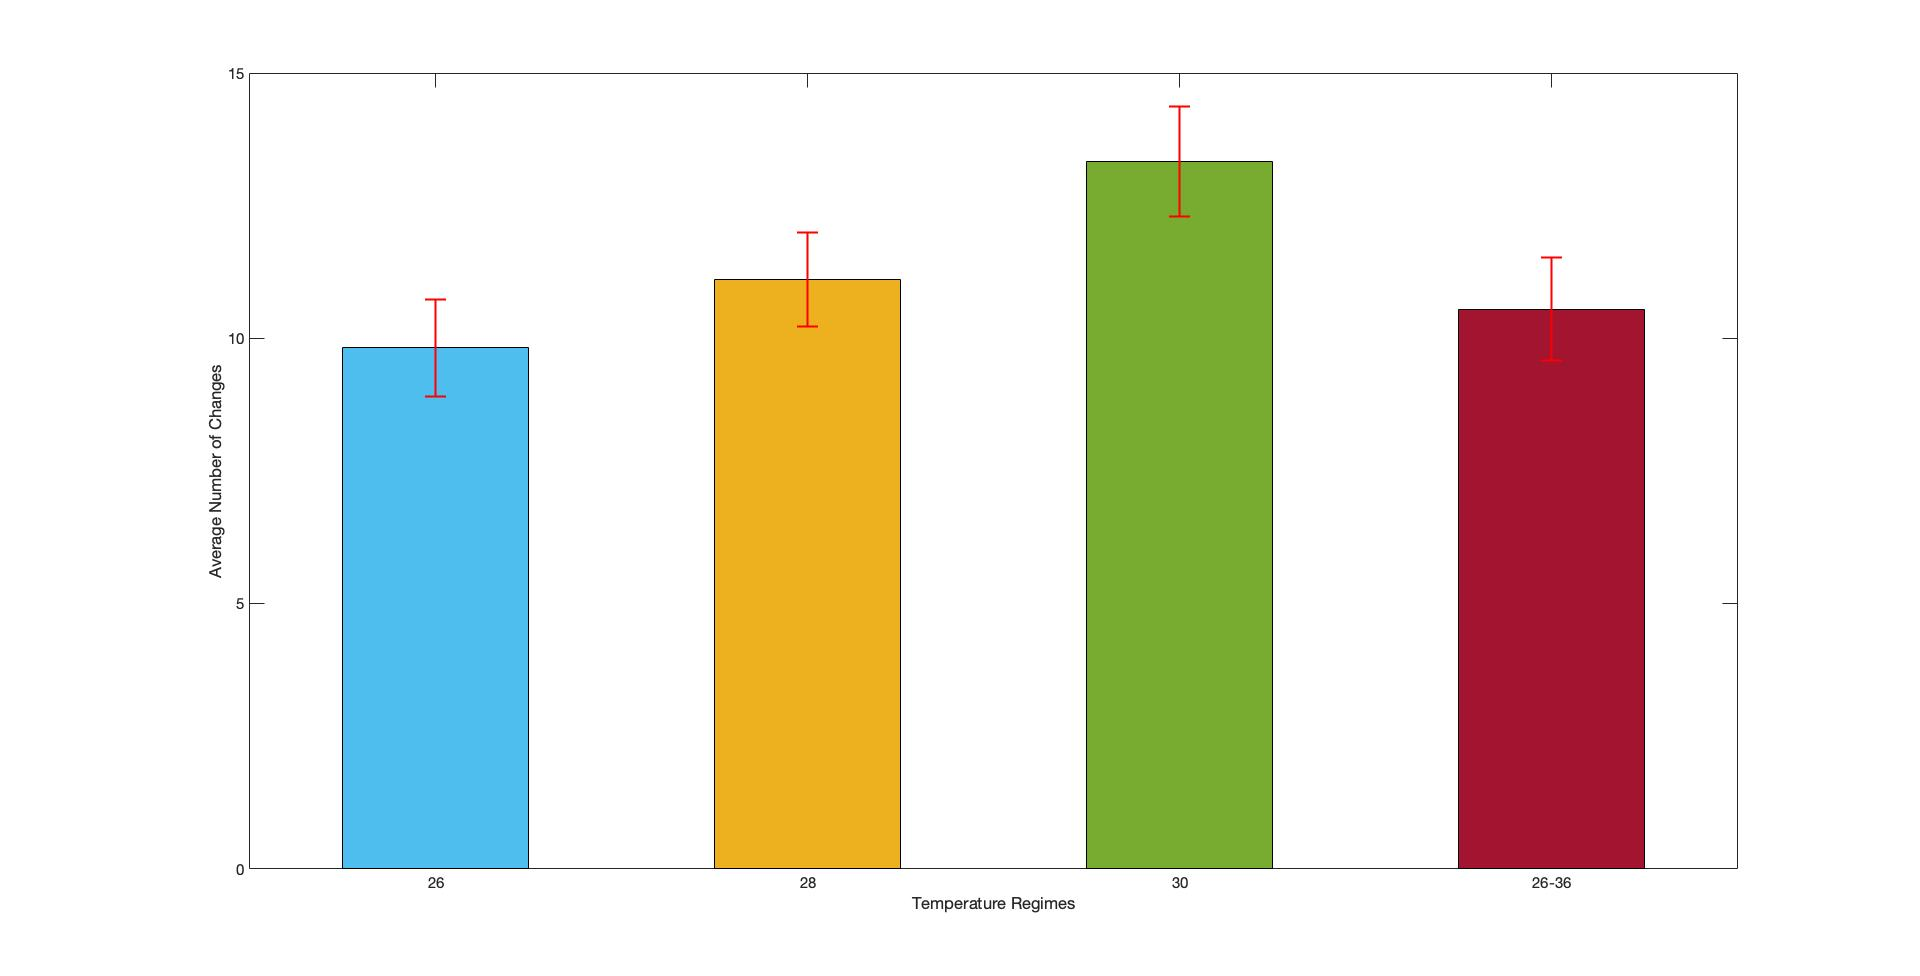
\includegraphics[width=\textwidth]{graph.jpg}
  \fbox{\begin{minipage}{50em}\text{}
    \begin{enumerate}
      \item What was the mean \(\pm \) standard error of coral growth (= change mg/cm2) at each of the four temperature categories?
      \begin{itemize}
        \item~~\quad{\(\ONE\C \)}~=~\BOX{\boxed{09.82~(mg/cm^2)~\pm~0.91}}{R}
        \item~~\quad{\(\TWO\C \)}~=~\BOX{\boxed{11.10~(mg/cm^2)~\pm~0.89}}{G}
        \item~~\quad{\(\THR\C \)}~=~\BOX{\boxed{13.33~(mg/cm^2)~\pm~1.04}}{B}
        \item \(\FOR\C \)~=~\BOX{\boxed{10.55~(mg/cm^2)~\pm~0.98}}{A}
      \end{itemize}
      \item What would happen if global climate change causes the average seawater temperature to increase to 30?
      \begin{itemize}
        \item
      \end{itemize}
      \text{}
    \end{enumerate}
  \end{minipage}}
\end{center}
\end{document}
